% {{{ PREABLE
\documentclass[12pt]{article}
\usepackage{sbc-template}
\usepackage[utf8]{inputenc}
\usepackage{graphicx,xurl}
\usepackage[T1]{fontenc} % avoid using two chars when special/accented letters
\usepackage[brazil]{babel}
\usepackage{xcolor}
\usepackage{listings}
\usepackage{colortbl}
\usepackage{multirow}
\usepackage{listings}
\usepackage{listingsutf8}
\usepackage{booktabs}
\usepackage{caption}
\usepackage{amsmath}
\usepackage[hidelinks]{hyperref} % hiden links inside the document - obrigatório LaTeX 2022
\usepackage[braket, qm]{qcircuit}
\usepackage{caption}
\usepackage{subcaption}
\usepackage{tikz}
%\usepackage{float} <- Não vamos usar este pacote!

\lstset{
  language=Python,                    
  basicstyle=\ttfamily\scriptsize,          
  numbers=left,                       
  numberstyle=\tiny\color{gray},       
  stepnumber=1,                       
  numbersep=5pt,                      
  backgroundcolor=\color{white},      
  showspaces=false,                   
  showstringspaces=false,             
  showtabs=false,                     
  frame=single,                       
  rulecolor=\color{black},            
  tabsize=2,                          
  captionpos=b,                       
  breaklines=true,                    
  keywordstyle=\color{blue},           
  commentstyle=\bfseries\color{black},
  stringstyle=\color{red},             
}

\sloppy
\title{Uma Proposta de Solução do Problema 3-SAT em Computação Quântica Usando Qiskit}

\author{Ricardo G. M. S. Ruiz\inst{1}, Gabriel A. R. Gomes\inst{1}, Calebe P. Bianchini\inst{1}}

\address{Faculdade de Computação e Informática\\
Universidade Presbiteriana Mackenzie\\
São Paulo -- SP -- Brasil
    \email{\{10389321, 10389313\}@mackenzista.com.br,
  calebe.bianchini@mackenzie.br}
}

\begin{document}

\maketitle

\begin{abstract}
    This meta-article aims to explore a quantum circuit approach to solving the classic and costly satisfiability problem, using the infamous Grover’s algorithm as the main resolution algorithm. In conjunction with the use of the Qiskit library, the article discusses a practical approach that implements the solution to the problem.
\end{abstract} 
\begin{resumo} 
  Este meta-artigo visa explorar uma abordagem de circuitos quânticos para a resolução do clássico e custoso problema da satisfabilidade, utilizando como principal algoritmo de resolução o famigerado algoritmo de Grover. Em conjunto com a utilização da biblioteca Qiskit, o artigo discorre sobre uma abordagem prática que implementa a solução para o problema.
\end{resumo}


\section{Introdução}

O constante avanço da computação e a crescente demanda por soluções mais eficientes têm conduzido a um cenário de busca contínua por algoritmos que otimizem a resolução de problemas complexos. Tanto na ciência e na produção de hardware quanto no mercado de trabalho, algoritmos clássicos têm sido pilares fundamentais para uma ampla gama de aplicações. No entanto, o advento da computação quântica promete revolucionar a forma como abordamos essas questões, oferecendo um novo paradigma de processamento que pode superar as limitações dos algoritmos clássicos em determinados contextos e superar o limite físico apresentado nos computadores atuais. Enquanto a computação clássica utiliza bits que podem estar em estados 0 ou 1, a computação quântica utiliza qubits que podem existir em estados de sobreposição, representando simultaneamente 0 e 1. Essa capacidade de processamento não determinístico é o que confere à computação quântica sua notável vantagem em certos tipos de cálculos. k-SAT é um desafio importante na ciência da computação que apresenta grandes questões ainda não descobertas, e, portanto, foi escolhido para ser desbravado no artigo em questão.


Este trabalho, fundamentado nos pontos discutidos, tem como objetivo propor um diagrama de circuito para resolver a expressão em FNC apresentada conforme a equação \ref{eq:expressao_fcn}. Ademais, pretende construir e testar um circuito quântico utilizando a biblioteca \textit{qiskit}, além de comparar os resultados obtidos para confirmar se a solução encontrada é ótima. A fim de alcançar esses objetivos, a seção \ref{sec:teorico} expõe os princípios teóricos empregados na elaboração do trabalho, com o fito de estabelecer as bases para uma compreensão clara da proposta em discussão. Em sequência, a seção \ref{sec:relacionados} apresenta as soluções de diversas pesquisas que buscam resolver o complexo problema da satisfação, por sua vez empregadas para elaborar a proposta final apresentada. Logo após, a seção \ref{sec:metodologia} detalha como os trabalhos citados contribuiram para a solução do circuito, as decisões tomadas durante a elaboração deste e, enfim, apresenta o circuito finalizado, que é seguido pela seção \ref{sec:resultados}, onde se realiza a execução do circuito e os resultados são comparados com os de uma tabela verdade. Por último, a seção \ref{sec:conclusoes} desenvolve uma conclusão sobre a solução obtida, e reforça a conclusão dos propósitos apresentados, incluindo então ideias para trabalhos futuros.


\section{Referencial Teórico}\label{sec:teorico}
%%%%% -> Fundamentos dos assuntos usados na construção do trabalho...

Antes de entrar na implementação proposta, é necessário o entendimento de alguns conceitos da computação clássica, como: Máquina de Turing, problema NP, k-SAT, e demais conceitos da computação quântica, como Algoritmo de Grover e Porta Hadamard.

A Máquina de Turing é um modelo abstrato de computação que utiliza uma fita infinita dividida em células discretas para manipular símbolos com base em regras definidas. Apesar de sua simplicidade, esse modelo é capaz de executar qualquer algoritmo computacional. A máquina consiste em uma cabeça que percorre a fita, podendo ler e escrever símbolos em cada célula. Cada célula contém um símbolo retirado de um conjunto finito de símbolos. Além disso, a máquina opera em um conjunto finito de estados. No início, a fita contém apenas a sequência de entrada e está vazia em todos os outros lugares. Caso a máquina precise armazenar informações, ela pode escrevê-las na fita. Para ler as informações escritas, a máquina pode mover sua cabeça de volta sobre elas. A computação continua até que a máquina decida produzir uma saída. As saídas ``aceitar'' e ``rejeitar'' são determinadas ao entrar em estados especificamente designados para tal. Caso não entre em nenhum estado de aceitação ou rejeição, a máquina continuará indefinidamente, sem parar.

Os problemas NP são aqueles para os quais, dada uma solução, é possível verificar, no pior caso,  utilizando uma Máquina de Turing não determinística, em tempo limitado polinomial \cite{sipser:07}. Acontece que, para determinados problemas, ao executar esse mesmo problema só que em uma máquina de turing determinística, obtemos um tempo limitado não polinomialmente. Por conta disso, os problemas NP são considerados os mais custosos de serem resolvidos computacionalmente, e, especialmente em seu pior caso, e, por conta disto, apresentam uma grande importância na teoria da computação.

Compreendendo o conceito de problema NP, é possível chegar no tema sobre o problema de satisfabilidade, e detalhar sua característica. O problema SAT é um dilema combinatório de grande relevância teórica e prática. Assim como outros problemas combinatórios, a busca por uma solução consome tempo, e esse tempo aumenta de maneira exponencial conforme o tamanho das entradas. Esse problema foi um dos primeiros a ser reconhecido como NP-Completo \cite{cook:71}, possuindo uma complexidade de $O(2^n)$. Seja \(x_1, \ldots, x_n\) variáveis booleanas, um literal pode ser uma variável booleana \(x_1\) ou sua negação \(\neg x_1\). Uma fórmula $k$-FNC (Forma Normal Conjuntiva) é uma conjunção de cláusulas, onde cada cláusula é uma disjunção de exatamente $k$ literais. O problema $k$-SAT é dado um $k$-FNC, decidir se é satisfazível ou não.

O algoritmo de Grover \cite{grover:96} é um método quântico para buscar um elemento alvo em um banco de dados não ordenado, e é significativamente mais rápido do que qualquer algoritmo clássico para o mesmo problema, apresentando uma complexidade de $O(\sqrt{N})$. Sua aplicação é descrita por meio de um difusor descrito por Grover conforme a equação
\ref{eq:grover}, onde $F$ representa a porta Hadamard, comumente utilizada para colocar o sistema em sobreposição, e $R$, uma matriz diagonal
\begin{equation}
D = FRF \label{eq:grover}
\end{equation}
é necessário entender que, para implementar o mesmo, o estado da arte define o uso de operadores de sobreposição quântica , como no caso da porta de Hadamard.\cite{silva:18} O termo Hadamard se refere à geração de bits aleatórios. O Hadamard, neste contexto, está relacionado à Transformada de Hadamard, que é uma operação linear fundamental em computação quântica. Ela é usada para criar superposições de estados quânticos, permitindo que um qubit esteja em uma combinação de estados $0$ e $1$ simultaneamente. Isso é crucial para algoritmos quânticos, como a geração de números aleatórios, pois permite explorar o paralelismo quântico e realizar cálculos em muitos estados possíveis ao mesmo tempo. A Transformada de Hadamard é representada por uma matriz específica que, quando aplicada a um vetor de estado de um qubit, resulta na superposição desejada de estados.

Com base no entendimento dos conteúdos citados, é possível desenvolver uma discussão sobre as propostas apresentadas no artigo para a solução do problema em questão.

\section{Trabalhos Relacionados}\label{sec:relacionados}
%%%%% -> Outros trabalhos, de outros autores, que fazem "a mesma coisa" que nós!
%% Dica: RESUMO de 4-6 parágrafos de cada artigo relacionado
%% Dica2: no "último" parágrafo da seção, apresentar uma correlação entre os trabalhos relacionados e o nosso trabalho

Para embasar este trabalho e identificar estudos relacionados relevantes, foi realizada uma pesquisa na base de dados Scopus, uma das mais abrangentes para artigos acadêmicos e publicações científicas. A consulta foi feita utilizando a seguinte query: \textit{``k-sat AND quantum AND computing AND grover''}, considerando o período de 2019 a 2024\footnote{Data da consulta: 08 de setembro de 2024.}. Essa busca resultou em 65 trabalhos.


Primeiramente, foi realizado uma filtragem com base em três principais categorias que podem ser categorizadas entre \textit{sim} e \textit{não}, sendo elas:
\begin{enumerate}
    \item  Se o trabalho encontrado pertence a categoria ``Título'', onde é categorizado se o título apresenta qualquer relação com computação quântica e o problema da satisfabilidade;
    \item Se o  trabalho encontrado pertence a categoria ``Grover'', que categoriza se o trabalho utiliza o algoritmo de Grover como metodologia para a resolução do problema;
    \item Se trabalho encontrado pertence a categoria ``$k$-SAT'', que afirma  para validar que o trabalho está resolvendo o mesmo problema em questão.
\end{enumerate}

Ao conduzir o processo de filtragem inicial, foram identificados e selecionados 17 trabalhos relevantes dentro do escopo proposto. Em seguida, foi realizada uma triagem detalhada e rigorosa, que consistiu na leitura minuciosa das introduções e conclusões de cada trabalho. Esse procedimento visou avaliar com maior precisão a pertinência e a relevância dos estudos em relação às questões centrais abordadas no presente artigo. Como resultado dessa análise aprofundada, o conjunto inicial foi reduzido a um total de 6 estudos, os quais representam as contribuições mais significativas para a fundamentação teórica e metodológica desta pesquisa, sendo apresentados de forma organizada na Tabela \ref{tab:trabalhos_relevantes}.

\begin{table}[h!]
\centering
\begin{tabular}{|p{5cm}|c|c|c|c|}
\hline
\textbf{Trabalho} & \textbf{Título} & \textbf{Grover} & \textbf{Quantum} & \textbf{$k$-SAT} \\
\hline
\cite{yang:23} & Sim & Não & Sim & Sim \\
\hline
\cite{parallelAndDistributed} & Não & Não & Sim & Sim \\
\hline
\cite{varmantchaonala:23} & Sim & Sim & Sim & Sim \\
\hline
\cite{wang:20} & Sim & Sim & Sim & Sim \\
\hline
\cite{mandl:24} & Sim & Não & Sim & Não\\
\hline
\cite{piro:20} & Sim & Sim & Sim & Sim\\
\hline
\end{tabular}
\caption{Categorias de filtragem}
\label{tab:trabalhos_relevantes}
\end{table}

%%RELACIONADO 1


%%RELACIONADO 2
Assim como em \cite{parallelAndDistributed}, é explicado que, a maneira mais comum de se resolver um problema k-SAT por meio da computação quântica, seria um circuito composto em dois principais componentes: um oráculo, e um difusor, onde o oráculo seria a nossa entrada, que visa responder ``sim'' ou ``não'' para o nosso problema, e o difusor se encaminha de maximizar a probabilidade de se obter o resultado esperado ao medir o estado dos \textit{qubits}.No estudo em questão, é introduzido a forma mais comum de se criar um oráculo para uma expressão lógica em FNC, que para dado uma fórmula $
\mathcal {F}: (a) \wedge (\overline{a} \vee b) \wedge (\overline{a} \vee c)
$, tendo como três variáveis \textit{booleanas} $a=1, b=1, c=1$, existe um oráculo ${U}$ composta por três blocos conectados entre si $C_1, C_2, C_3$ onde $C_1$ visa processar a primeira cláusula $(a)$, $C_2$ processa a segunda cláusula
$(\overline{a} \vee b)$, e por fim $C_3$ processa a terceira $(\overline{a} \vee c)$, onde são processadas de forma sequencial devido ao fato de todas cláusulas dependerem da variável $a$.
Cada cláusula por sua vez é composta por portas $M_j$, onde cada um representa literal $l_j$, onde caso $l_j$ seja uma negação, é inferido uma porta $X$, caso o contrário, uma porta identidade $I$. O qubit obtido então representa o valor da cláusula $C_1$. Após a junção das cláusulas é obtido assim um bloco correspondente forma geral $\omega$ apresentado na figura \ref{fig:oraculo_forma_geral}. Após a construção de todos os circuitos, eles são conectados por uma porta CNOT. (bloco $\wedge$), seguido por uma porta $Z$, e, por fim, é implementado o bloco $\Omega ^{-1}$, que representa a operação inversa de $\Omega$ a fim de restaurar o estado do vetor de entrada.

\begin{figure}[ht]
\centering
\scalebox{0.77}{
\begin{tikzpicture}
    \node (qc) at (0,0) {
        \Qcircuit @C=0.6em @R=0.2em @!R {
            & & & C_1 & & & C_2 & & & C_3 & & \land & P\\
            \nghost{a :  } & \lstick{a :  } & \gate{X} & \ctrl{1} & \gate{X} & \qw & \ctrl{3} & \qw & \qw & \ctrl{4} & \qw & \qw & \qw & \qw & \qw & \ctrl{4} & \qw & \qw & \ctrl{3} & \qw & \gate{X} & \ctrl{1} & \gate{X}\\
            \nghost{C_{1_\textit{ancilla}} :  } & \lstick{C_{1_\textit{ancilla}} :  } & \gate{X} & \targ & \qw & \qw & \qw & \qw & \qw & \qw & \qw & \ctrl{2} & \qw & \ctrl{2} & \qw & \qw & \qw & \qw & \qw & \qw & \qw & \targ & \gate{X}\\
            \nghost{b :  } & \lstick{b :  } & \qw & \qw & \qw & \gate{X} & \ctrl{1} & \gate{X} & \qw & \qw & \qw & \qw & \qw & \qw & \qw & \qw & \qw & \gate{X} & \ctrl{1} & \gate{X} & \qw & \qw & \qw\\
            \nghost{C_{2_\textit{ancilla}} :  } & \lstick{C_{2_\textit{ancilla}} :  } & \qw & \qw & \qw & \gate{X} & \targ & \qw & \qw & \qw & \qw & \ctrl{2} & \qw & \ctrl{2} & \qw & \qw & \qw & \qw & \targ & \gate{X} & \qw & \qw & \qw\\
            \nghost{c :  } & \lstick{c :  } & \qw & \qw & \qw & \qw & \qw & \qw & \gate{X} & \ctrl{1} & \gate{X} & \qw & \qw & \qw & \gate{X} & \ctrl{1} & \gate{X} & \qw & \qw & \qw & \qw & \qw & \qw\\
            \nghost{C_{3_\textit{ancilla}} :  } & \lstick{C_{3_\textit{ancilla}} :  }& \qw & \qw & \qw & \qw & \qw & \qw & \gate{X} & \targ & \qw & \ctrl{1} & \qw & \ctrl{1} & \qw & \targ & \gate{X} & \qw & \qw & \qw & \qw & \qw & \qw\\
            \nghost{F :  } & \lstick{F :  } & \qw & \qw & \qw & \qw & \qw & \qw & \qw & \qw & \qw & \targ & \gate{Z} & \targ & \qw & \qw & \qw & \qw & \qw & \qw & \qw & \qw & \qw\\
            & & & & & & & \Omega & & & & & & & & & & \Omega^{-1}
        }
    };
    \draw[dashed, thick] (-7, 2.28) rectangle (-4.67, 0.85);
    \draw[dashed, thick] (-4.58, 2.28) rectangle (-2.30, -0.35);
    \draw[dashed, thick] (-2.21, 2.28) rectangle (0.04, -1.6);
    \draw[dashed, thick] (0.16, 2.28) rectangle (0.66, -2.2);
    \draw[dashed, thick] (0.76, 2.28) rectangle (1.48, -2.2);
\end{tikzpicture}
}
\caption{Forma geral do oráculo baseado em \cite{parallelAndDistributed}}
\label{fig:oraculo_forma_geral}
\end{figure}

Alguns trabalhos visam não apenas propor uma resolução para o clássico problema da satisfabilidade, como também realizar otimizações que reduzem a quantidade de qubits totais de um circuito quântico SAT, como em \cite{yang:23} onde além de propor um algoritmo para a criação de uma oráculo, também é feito uma redução  na quantidade de qubits \textit{ancilla} existentes em um SAT-oráculo, que podem ser definidos como \textit{qubits} extras incorporados no circuito a fim de armazenar o resultado de cada disjunção de uma expressão FCN. O trabalho menciona que, para construir uma oráculo para uma dada expressão em FNC, é comumente utilizado uma quantidade de qubits \textit{ancilla} de \( 2m - 1 \), sendo $m$ a quantidade de cláusulas da expressão em questão. O artigo sugere uma solução para diminuir o uso e a utilização de recursos computacionais quânticos, ao propor um oráculo com quantidade ajustável de qubits \textit{ancilla}, recurso especialmente útil para circuitos que resolvem expressões com centenas (ou senão milhares) de cláusulas.
O estudo em questão começa com a explicação do que são e do motivo pelo qual devemos empregar oráculos em circuitos quânticos, e, juntamente com a explicação do problema SAT, enfatiza-se teoricamente como esses oráculos devem ser utilizados em circuitos que visam resolver o problema da satisfabilidade, reforçando a falha dos algoritmos convencionais quando o assunto é a limitação da quantidade de qubit \textit{ancilla}
Após o uso de um algoritmo que possibilita a limitação da quantidade de \textit{qubits ancilla}, é implementado o oráculo de forma prática, e, então é explicado que a expressão proposta pode ser satisfeita através da aplicação do algoritmo de Grover.

Conforme explicado anteriormente, uma forma geral para um circuito que visa resolver o problema do 3-SAT pode ser apresentado através de um oráculo que representa uma expressão FNC, e um difusor que amplifica e realizar a busca exaustiva do resultado da expressão apresentada. Em \cite{wang:20} O artigo cita a vantagem de utilizar Grover por conta de sua complexidade $O \left( \sqrt{N} \right)$ em uma busca não estruturada em uma base de dados. Munido deste conhecimento, o estudo além de montar um oráculo que representa uma expressão em FNC, também apresenta a viabilidade do uso do algoritmo de Grover como difusor. Também é explicado que tal abordagem permite que a complexidade total do circuito seja equivalente a $O(2^{n/2})$. Assim como no trabalho citado anteriormente, o circuito consiste na montagem de um oráculo representante da expressão em FNC, e logo em seguida uma amplificação com um difusor (nesse caso específico, o algoritmo de Grover) a fim de realizar a busca exaustiva pelas soluções satisfatórias da expressão em questão.

%%RELACIONADO 4
Cabe-se ressaltar que os trabalhos relacionados citados até então introduzem uma solução que consiste em três principais etapas: 1. Criação de um oráculo que representa a expressão FNC para o estado inicial, 2. Sobreposição uniforme de estados das cláusulas representadas por cada qubit 3. Em conjunto com o algoritmo de Grover, é realizado uma busca exaustiva no espaço de busca em conjunto. (veja a figura \ref{fig:diagrama_fluxo_trabalhos_relacionados}). 

\begin{figure}[h]
    \centering
    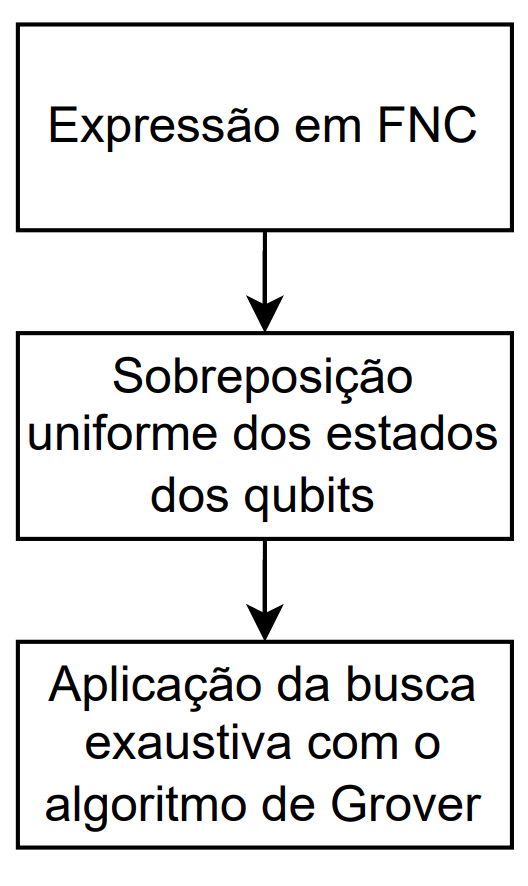
\includegraphics[width=0.18\linewidth]{diagrama_fluxo_convencional_trabalhos_relacionados.png}
        \caption{Diagrama de fluxo da montagem dos circuitos apresentados até então}
        \label{fig:diagrama_fluxo_trabalhos_relacionados}
\end{figure}
A este ponto, vale citar outros trabalhos que visam acabar com essa abordagem custosa e apresentar melhorias, como em \cite{varmantchaonala:23}, onde, através de um algoritmo proposto no trabalho, é realizado uma subdivisão do estado inicial, que, conforme citado anteriormente e nos outros trabalhos já é computado exaustivamente com o algoritmo de Grover. Ao invés disso, e de forma não uniforme, é feito uma aplicação de divisão em conquista que visa realizar uma sobreposição de parte do espaço de busca, contando com apenas os valores que são potencialmente uma solução ótima. Tal proposta não uniforme e baseada em divisão em conquista apresenta uma execução do algoritmo de Grover com complexidade
$O \left( \sqrt{{N/S}} \right)$, de sendo $N$ o número de potenciais soluções, e $S$ o fator de redução/subdivisão de espaço utilizado pelo algoritmo. Trazendo uma complexidade relativamente superior ao algoritmo de Grover, que em seu estado da arte, e em conjunto com os métodos uniformes citados anteriormente, apresenta uma complexidade de $O \left( \sqrt{N} \right)$. No próprio trabalho em questão, também é citado que existem outras maneiras de solucionar o problema do SAT de forma não determinística, mas sim do uso de meta heuristicas, como através da utilização de QAOA (\textit{Quantum Approximate Optimization Algorithm}). Adentrando nessa descoberta, outros trabalhos que utilizam tal \textit{approach} são dignos de serem citados.

%%RELACIONADO 5

Da mesma forma que brevemente citado no trabalho explicado anteriormente, em \cite{mandl:24}, é apresentado um algoritmo visado ao uso de meta heurísticas para a solução do problema MAX-3SAT(uma generalização do problema SAT), mais em específico o QAOA (\textit{Quantum Approximate Optimization Algorithm}), um algoritmo quântico utilizado para resolver problemas de otimização combinatória, que em sua essência procura encontrar os estados com autovalor mínimo de um dado operador Hamiltoniano $H_C$. Através de uma \textit{ansatz} modelada para o problema a ser resolvido que pode ser resumida em circuito em seu estado inicial seguido por $p$ repetições que concatenam um operador de separação de fase $U(H_C,\gamma_i)$ e um circuito \textit{mixer} $U(H_B, \beta_i)$. Tal arranjo permite a identificação de um conjunto solução para o problema.


%%RELACIONADO 6
Por fim, o artigo \cite{piro:20} avalia a aplicação de computação quântica para a solução de instâncias arbitrárias do problema Exactly-1 K-SAT e mostra as melhorias que são proporcionadas por um solucionador quântico. O problema Exactly-1 K-SAT consiste em encontrar uma atribuição satisfatória na qual exatamente um literal é verdadeiro em cada cláusula. Este trabalho realiza uma generalização de outro solucionador quântico que resolve o problema Exactly-1 3-SAT utilizando o algoritmo de Grover, essa generalização é feita em três etapas:
\begin{enumerate}
    \item Inicialização onde é aplicado portas Hadamard para cada variável e para a saída;
    \item Etapa de codificação do problema onde cada cláusula é codificada no circuito usando portas que permitem inverter o qubit correspondente à cláusula se ela tiver exatamente um literal verdadeiro;
    \item Inversão sobre a média onde foi modificado os coeficientes correspondentes à solução correta aplicando a operação unitária \(W\):
\end{enumerate} 
\[
W = \big( - \overset{n}{\bigotimes} \mathcal{H} \big) D \big( \overset{n}{\bigotimes} \mathcal{H} \big)
\]



%%VAMOS RESUMIR CADA UM, DEPOIS DAR UM TAPA EJUNTAR TUDO
%%ESTRUTURA: [ANCILLA], [ORACULO], [AMPLITUDE AMPLIFIER - GROVER], 


%%COMO AJUDOU?
\section{Metodologia}\label{sec:metodologia}
%%%%% -> Como fizemos o trabalho até o momento?
%%%%% -> Como continuaremos?
Para adentrar na abordagem prática para a resolução do problema, foi feito 
um breve estudo sobre como utilizar a biblioteca \textit{Qiskit}, ferramenta altamente utilizada para 
desenvolvimento e execução de circuitos quânticos. Em consonância com o 
conteúdo exposto no livro \cite{silva:18}, foi empreendido um estudo 
aprofundado sobre circuitos quânticos. Tal investigação permitiu não apenas 
a compreensão das complexidades teóricas, mas também a aplicação prática dos 
conceitos abordados. Adicionalmente, foi conduzida uma análise rigorosa 
sobre a implementação do algoritmo de Grover, conforme delineado no trabalho 
de \cite{gamberi:22}. Essa investigação possibilitou a atualização do 
procedimento para a versão mais recente do \textit{Qiskit}, considerando que este empregava uma versão anterior da 
biblioteca em questão. 

Na sequência do estudo sobre a base do que foi estudado, procedeu-se à análise de quais algoritmos e estruturas de circuitos deveriam ser utilizadas na formulação do circuito proposto. Dentre as abordagens estudas, cabe-se citar as mesmas propostas em \cite{mandl:24}, que conforme explicado anteriormente consiste no uso de meta heurísticas e aplicações matemáticas para a criação de um circuito que analisa as possibilidades do problema MAX 3-SAT, o trabalho feito em \cite{fernandes:19}, \cite{parallelAndDistributed} e \cite{wang:20}, que ao invés do uso de meta-heurísticas, uma abordagem determinística é apresentada, uma vez que ao invés de se basear em um evento probabilístico, as abordagens em questão apresentam uma busca exaustiva pelo resultado a fim de determinar a solução ótima.

Após a definição de todas as abordagens já utilizadas em estudos e no estado da arte, foi necessário a escolha de qual dos métodos seria o mais interessante, simples, de fácil entendimento e prático para a montagem do circuito. Com isto em mente, foi determinado que a solução deveria seguir uma abordagem determinística, a fim de apresentar uma abordagem voltada ao desenvolvimento de \textit{software} apresentada pela mesma em contraste com uma abordagem matemática definida pelo uso de meta-heurísticas.

Em consonância com os trabalhos determinísticos estudados anteriormente, foi necessário entender primeiramente o diagrama do circuito que mais tarde seria portado e executado em um \textit{software}. Dentre os diagramas de circuitos apresentados nos trabalhos relacionados, foi escolhido a abordagem realizada por \cite{fernandes:19}, que, por mais que os demais outros trabalhos já citados apresentem uma possível solução mais eficiente, o mesmo foi escolhido devido ao fato de apresentar a solução original para o problema. O diagrama consiste nas mesmas etapas ilustradas na figura \ref{fig:diagrama_fluxo_trabalhos_relacionados}, onde o circuito é dividido em dois principais blocos: um oráculo que representa a expressão em FNC escolhida e um difusor composto por uma diagonal $\mathrm{\textit{D}_x}$ que se encaminha de maximizar a probabilidade de obter a solução ótima, conforme a figura \ref{fig:diagrama_oraculo_difusor}.


\begin{figure}[ht]
\centering
\scalebox{0.9}{
\Qcircuit @C=1.0em @R=0.2em @!R {
            n_{literais} & & & & & & & \mbox{\textit{Difusor}}\\
	 	\nghost{{x}_{1} :  } & \lstick{{q}_{1} \ket{0}:  } & \multigate{2}{\mathrm{\,\,\textit{H}^{{\bigoplus}n}}}& \qw  & \qw & \multigate{7}{Or\acute{a}culo}  & \qw & \multigate{2}{\mathrm{\,\,\textit{H}^{{\bigoplus}n}}} & \multigate{2}{\mathrm{\textit{D}_x}} & \multigate{2}{\mathrm{\,\,\textit{H}^{{\bigoplus}n}}} & \meter & \qw &\qw &\qw \\
	 	\nghost{{x}_{2} :  } & \lstick{... \ket{0}:  } & \ghost{\mathrm{\,\,\textit{H}^{{\bigoplus}n}}} & \qw & \qw & \ghost{Or\acute{a}culo} & \qw & \ghost{\mathrm{\,\,\textit{H}^{{\bigoplus}n}}} & \ghost{\mathrm{\textit{D}_x}} & \ghost{\mathrm{\,\,\textit{H}^{{\bigoplus}n}}} & \qw & \meter & \qw & \qw\\
	 	\nghost{{x}_{3} :  } & \lstick{{q}_{n} \ket{0}:  } & \ghost{\mathrm{\,\,\textit{H}^{{\bigoplus}n}}} & \qw & \qw & \ghost{Or\acute{a}culo} & \qw & \ghost{\mathrm{\,\,\textit{H}^{{\bigoplus}n}}} & \ghost{\mathrm{\textit{D}_x}} & \ghost{\mathrm{\,\,\textit{H}^{{\bigoplus}n}}} & \qw & \qw & \meter & \qw\\
            k_{cl\acute{a}usulas} & & & & & & & & \\
	 	\nghost{{q}_{3} :  } & \lstick{{a}_{1} \ket{0}:  } & \qw & \qw & \qw & \ghost{Or\acute{a}culo} & \qw & \qw & \qw & \qw & \qw & \qw & \qw & \qw\\
	 	\nghost{{q}_{4} :  } & \lstick{... \ket{0}:  } & \qw & \qw & \qw & \ghost{Or\acute{a}culo} & \qw & \qw & \qw & \qw & \qw & \qw & \qw & \qw\\
	 	\nghost{{q}_{5} :  } & \lstick{{a}_{k} \ket{0}:  } & \qw & \qw & \qw & \ghost{Or\acute{a}culo} & \qw & \qw & \qw & \qw & \qw & \qw & \qw & \qw\\
	 	\nghost{{q}_{6} :  } & \lstick{{a}_{sa\acute{\imath}da}  \ket{0}:  } & \gate{\mathrm{\textit{H}}} & \gate{\mathrm{\textit{Z}}} & \qw & \ghost{Or\acute{a}culo} & \qw & \qw & \qw & \qw & \qw & \qw & \qw &\qw
   \gategroup{2}{8}{4}{10}{.8em}{--}
   \inputgroupv{2}{4}{.8em}{.8em}{} \inputgroupv{6}{8}{.8em}{.8em}{}
}}
\caption{Diagrama para um circuito resolvedor 3-SAT por meio de um oráculo e um difusor}
\label{fig:diagrama_oraculo_difusor}
\end{figure}


Com o diagrama geral do circuito em mãos, os próximos passos foram: 1. Criar um oráculo e 2. Definir e criar um difusor:

Para o oráculo. foi feito um estudo baseado nos trabalhos de \cite{fernandes2:19}, \cite{fernandes:19}, \cite{parallelAndDistributed}, que descorrem sobre maneiras de se construir a mesma através de uma dada expressão em FNC (veja a figura \ref{fig:oraculo_forma_geral}. Desta forma, para a implementação da mesma, foi criado um circuito que representa a expressão FNC conforme a equação \ref{eq:expressao_fcn}.
\begin{equation}
(\neg A \lor \neg B \lor \neg C) \land (A \lor \neg B \lor C) \land (A \lor B \lor \neg C)\label{eq:expressao_fcn}
\end{equation}
Em relação a quantidade de \textit{qubits}, é possível definir conforme a equação \ref{eq:qtd_qubits}, 
\begin{equation}
qtd_{\textit{qubits}} = n + k + 1\label{eq:qtd_qubits}
\end{equation}
onde $n$ representada a quantidade de literais, $k$ a quantidade de cláusulas, e $qtd_{\textit{qubits}}$ a quantidade de \textit{qubits} do circuito. Substituindo os valores conforme a equação \ref{eq:expressao_fcn}, obtemos um total de 3 literais e 3 cláusulas, ou seja, $n = 3$ e $k = 3$, e somando com mais um \textit{qubit} para armazenar o resultado conjunção das expressões, resultando portanto em um total de 7 \textit{qubits} para o circuito.

A principal ideia por trás dos \textit{qubits} adicionais (de acordo com a lógica da equação \ref{eq:qtd_qubits}, o valor de $k$) é servir como um \textit{ancilla} para armazenar o resultado da disjunção de cada cláusula, e portanto, precisamos de uma quantidade de \textit{qubits ancilla} equivalente a quantidade de cláusulas escolhidas. Desta forma, o principal objetivo de cada bloco de cláusula $C$ (figura \ref{fig:oraculo_forma_geral}), é representar a negação ou identidade de cada literal da disjunção em questão, e atribuir o resultado da disjunção em seu respectivo \textit{ancilla} por meio de uma porta Toffoli, onde cada literal é um \textit{qubit} de controle (onde seu estado (1/0) é representado caso haja negação ou não, respectivamente), e o \textit{qubit target} é seu respectivo \textit{ancilla}  (figura \ref{fig:expressao_toffoli}). Em sequência da montagem das cláusulas e a fim de representar a conjunção ($\land$), é colocado uma porta Toffoli que tem como controle os \textit{qubits} ancilla (em seus atuais estados), e como \textit{target} o \textit{qubit} extra separado anteriormente para a saída da expressão. 
Após este ponto, a ideia principal neste momento é reverter o circuito ao seu estado inicial. Tendo isto em mente, é construído outro bloco composto de portas Toffoli, só que agora representando o espelho da expressão montada anteriormente, isto é, a montagem de cada cláusula já feita, mas em ordem inversa. (veja a figura \ref{fig:expressao_toffoli_espelho}).

\begin{figure}[ht]
\centering
\begin{subfigure}{0.45\textwidth}
\Qcircuit @C=1.0em @R=0.2em @!R { \\
	 	\nghost{A :  } & \lstick{A :  } & \ctrl{1} & \ctrlo{1} & \ctrlo{1} &\qw\\
	 	\nghost{B :  } & \lstick{B :  } & \ctrl{1} & \ctrl{1} & \ctrlo{1} & \qw\\
	 	\nghost{C :  } & \lstick{C :  } & \ctrl{1} & \ctrlo{2} & \ctrl{3} & \qw\\
	 	\nghost{{a}_{A} :  } & \lstick{{a}_{A} :  } & \targ & \qw & \qw & \qw\\
	 	\nghost{{a}_{B} :  } & \lstick{{a}_{B} :  } & \qw & \targ & \qw & \qw\\
	 	\nghost{{a}_{C} :  } & \lstick{{a}_{C} :  } & \qw & \qw & \targ & \qw\\
\\ }
\caption{Circuito quântico para a equação \ref{eq:expressao_fcn}}
\label{fig:expressao_toffoli}
\end{subfigure}
\begin{subfigure}{0.45\textwidth}
\centering
\Qcircuit @C=1.0em @R=0.2em @!R { \\
	 	\nghost{A :  } & \lstick{A :  } & \ctrlo{1} & \ctrlo{1} & \ctrl{1} & \qw\\
	 	\nghost{B :  } & \lstick{B :  } & \ctrlo{1} & \ctrl{1} & \ctrl{1} &  \qw\\
	 	\nghost{C :  } & \lstick{C :  } & \ctrl{3} & \ctrlo{2} & \ctrl{1} & \qw\\
	 	\nghost{{a}_{A} :  } & \lstick{{a}_{A} :  } & \qw & \qw & \targ & \qw\\
	 	\nghost{{a}_{B} :  } & \lstick{{a}_{B} :  } & \qw & \targ & \qw & \qw\\
	 	\nghost{{a}_{C} :  } & \lstick{{a}_{C} :  } & \targ & \qw & \qw & \qw\\
\\ }
\caption{Simetria da equação \ref{eq:expressao_fcn}}
\label{fig:expressao_toffoli_espelho}
\end{subfigure}
\caption{Representação da montagem da expressão escolhida por meio de um circuito composto por portas Toffoli e qubits ancilla}
\end{figure}

Unindo todos os componentes citados anteriormente, é possível obter então o circuito final para o oráculo (veja a figura \ref{fig:oraculo_final})

\begin{figure}[ht]
\centering
\scalebox{0.9}{
\Qcircuit @C=1.0em @R=0.2em @!R { \\
   &&&&&& \text{Disjun\c{c}\~{a}o} &&&& \text{Conjun\c{c}\~{a}o} &&&& \text{Simetria} &&&&\\
	 	\nghost{A :  } & \lstick{A :  } & \qw & \qw & \qw & \ctrl{1} & \ctrlo{1} & \ctrlo{1} & \qw & \qw & \qw & \qw & \qw & \ctrlo{1} & \ctrlo{1} & \ctrl{1} & \qw & \qw & \qw \\
	 	\nghost{B :  } & \lstick{B :  } & \qw & \qw & \qw & \ctrl{1} & \ctrl{1} & \ctrlo{1} & \qw & \qw & \qw & \qw & \qw & \ctrlo{1} & \ctrl{1} & \ctrl{1} & \qw & \qw & \qw \\
	 	\nghost{C :  } & \lstick{C :  } & \qw & \qw & \qw & \ctrl{1} & \ctrlo{2} & \ctrl{3} & \qw & \qw & \qw & \qw & \qw & \ctrl{3} & \ctrlo{2} & \ctrl{1} & \qw & \qw & \qw \\
	 	\nghost{{a}_{A} :  } & \lstick{{a}_{A} :  } & \qw & \qw & \qw & \targ & \qw & \qw & \qw & \gate{\mathrm{X}} & \ctrl{1} & \gate{\mathrm{X}} & \qw & \qw & \qw & \targ & \qw & \qw & \qw \\
	 	\nghost{{a}_{B} :  } & \lstick{{a}_{B} :  } & \qw & \qw & \qw & \qw & \targ & \qw & \qw & \gate{\mathrm{X}} & \ctrl{1} & \gate{\mathrm{X}} & \qw & \qw & \targ & \qw & \qw & \qw & \qw \\
	 	\nghost{{a}_{C} :  } & \lstick{{a}_{C} :  } & \qw & \qw & \qw & \qw & \qw & \targ & \qw & \gate{\mathrm{X}} & \ctrl{1} & \gate{\mathrm{X}} & \qw & \targ & \qw & \qw & \qw & \qw & \qw \\
	 	\nghost{{a}_{sa\acute{\imath}da} :  } & \lstick{{a}_{sa\acute{\imath}da} :  } & \gate{\mathrm{H}} & \gate{\mathrm{Z}} & \qw & \qw & \qw & \qw & \qw & \qw & \targ & \qw & \qw & \qw & \qw & \qw & \qw & \qw & \qw
   \gategroup{3}{6}{8}{8}{.8em}{--}
   \gategroup{3}{10}{9}{12}{1.8em}{--}
   \gategroup{3}{14}{8}{16}{.8em}{--}
}}
\caption{Oráculo criado que representa a expressão FNC conforme a equação \ref{eq:expressao_fcn}}
\label{fig:oraculo_final}
\end{figure}

Após a implementação do oráculo, foi realizado um estudo para a implementação de um difusor a fim de seguir o estado da arte para implementar o algoritmo de Grover.
Da mesma forma que em \cite{gamberi:22}, foi aplicado o difusor como em seu estado da arte, definido conforme a equação \ref{eq:grover} sendo \textit{F} a aplicação da porta Hadamard (no caso para este trabalho, seria a aplicação  para os n \textit{qubits}), ou seja, $F = {H}^{{\bigoplus}n}$, e $D$ uma matriz diagonal definida por um vetor sendo o primeiro elemento igual a 1, e os demais assumem o valor de -1:\\
$D_{i,j} = 0$ se $i \neq j$ \\
$D_{i,i} = 1$, se $i = 0$ \\
$D_{i,i} = -1$, se $i \neq 0$ \\

Tendo em mente o diagrama do circuito proposto conforme a figura \ref{fig:diagrama_oraculo_difusor}, o próximo para a resolução do problema foi a criação do circuito. Para essa etapa, foi escolhido a linguagem de programação \textit{Python} em conjunto com a biblioteca \textit{Qiskit}.
O primeiro passo então foi a criação do oráculo, que em suma pode ser aplicada da mesma maneira como no bloco \ref{lst:create_oracle}
\begin{lstlisting}[language=Python, caption={Criação do oráculo}, frame=single, label={lst:create_oracle}]
def CreateOracle():
  qubit_qtd = clauses_qtd = 3
  register_qtd = qubit_qtd + clauses_qtd + 1

  qreg_q = QuantumRegister(register_qtd, 'q')
  creg_c = ClassicalRegister(qubit_qtd, 'c')
  qc = QuantumCircuit(qreg_q, creg_c)

  # Amplifica e inverte a fase do qubit de resultado
  qc.h(6)
  qc.z(6)
  qc.barrier()
  
  # Disjuncao (~A | ~B | ~C)
  qc.append(CXGate().control(num_ctrl_qubits=2, ctrl_state='11'), [0,1,2,3])
  # Disjuncao (A | ~B | C)
  qc.append(CXGate().control(num_ctrl_qubits=2, ctrl_state='00'), [0,2,1,4])
  # Disjuncao (A | B | ~C)
  qc.append(CXGate().control(num_ctrl_qubits=2, ctrl_state='00'), [0,1,2,5])

  # Conjuncao
  qc.barrier()
  qc.x(qreg_q[3])
  qc.x(qreg_q[4])
  qc.x(qreg_q[5])
  qc.append(CXGate().control(num_ctrl_qubits=2, ctrl_state='11'), [3,4,5,6])
  qc.x(qreg_q[3])
  qc.x(qreg_q[4])
  qc.x(qreg_q[5])
  qc.barrier()

  # Simetria (A | B | ~C)
  qc.append(CXGate().control(num_ctrl_qubits=2, ctrl_state='00'), [0,1,2,5])
  # Simetria  (A | ~B | C)
  qc.append(CXGate().control(num_ctrl_qubits=2, ctrl_state='00'), [0,2,1,4])
  # Simetria  (~A | ~B | ~C)
  qc.append(CXGate().control(num_ctrl_qubits=2, ctrl_state='11'), [0,1,2,3])

  qc.barrier()

  return qc
\end{lstlisting}
Com a criação do oráculo, os passos restantes se definem em: \\
1. Criação da diagonal (veja o trecho de código \ref{lst:create_diagonal})\\
2. Criação e anexo do difusor ao oráculo (veja o trecho de código \ref{lst:create_difusor})\\

\begin{lstlisting}[language=Python, caption={Criação da diagonal}, frame=single, label={lst:create_diagonal}]
def CreateDiagonalSequence(number, qubits):
    diagonalSize = pow(2,qubits)
    if (diagonalSize < number - 1): return -1
    aux = np.ones(diagonalSize, dtype=int)
    aux[number] = -1
    return aux

def GetDiagonal():
  # Quantidade de literais (A,B,C)
  qubit_qtd = 3
  groverDiagonal = list(CreateDiagonalSequence(0, qubit_qtd))
  
  # Instancia da diagonal disponibilizada pelo qisikit
  return Diagonal(groverDiagonal) 
\end{lstlisting}

\begin{lstlisting}[language=Python, caption={Adição do operador de Grover ao \textit{oráculo}}, frame=single, label={lst:create_difusor}]
def ApplyGrover(oracle):
  num_qubits = 7
  qr = QuantumRegister(num_qubits)
  qc = QuantumCircuit(qr, name)
  qubits = [0,1,2,3,4,5,6]
  qc.compose(oracle, qubits, inplace=True)

  # Aplica Hadamart Para cada qubit queremos medir
  qc.h(0)
  qc.h(1)
  qc.h(2)

  #Aplica a diagonal para os 3 qubits que desejamos medir
  qc.compose(
      GetDiagonal(oracle),qubits=[0,1,2], inplace=True
  )
  # Aplica Hadamart Para cada qubit que queremos medir
  qc.h(0)
  qc.h(1)
  qc.h(2)

  return qc
\end{lstlisting}

Com a aplicação de Hadamard nos 3 primeiros \textit{qubits} (literais), e a incluindo a medição dos mesmos, o circuito final então é obtido (veja a figura \ref{fig:circuito_final})

\begin{figure}[ht]
    \centering
    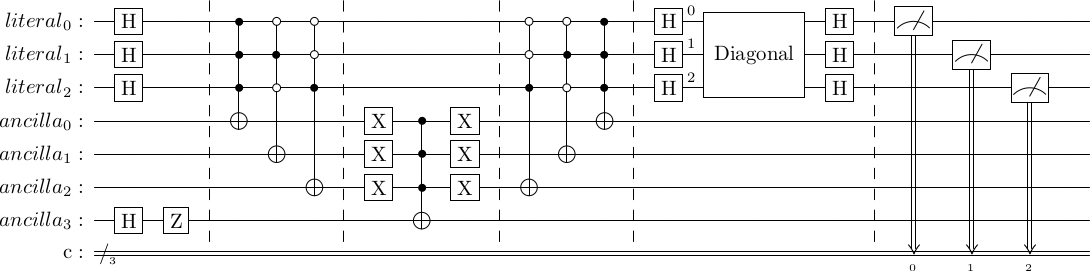
\includegraphics[width=1\linewidth]{circuito_final.png}
    \caption{Circuito final}
    \label{fig:circuito_final}
\end{figure}

\section{Resultados obtidos}\label{sec:resultados}

Conforme explicitado anteriormente, foi criado o circuito quântico na figura \ref{fig:circuito_final} que visa solucionar a expressão FNC \ref{eq:expressao_fcn}.

Executando o circuito obtido, é possível gerar o histograma presente na figura \ref{fig:histograma_circuito}, que representa as atribuições (1/0) dos valores de C, B e A que resultam em não satisfação para a expressão \ref{eq:expressao_fcn}.
No caso em questão, os valores 000, 001, 011, 101, 110 representam as atribuições de C,B,A, respectivamente para a obtenção da satisfabilidade.

Sendo assim, as atribuições com maior probabilidade indicam os valores de C, B e A que levam a um resultado booleano de "falso", enquanto as com menor probabilidade correspondem às atribuições que resultam no valor booleano de "verdadeiro" para a expressão.

\begin{figure}
\centering
    \begin{subfigure}{0.4\textwidth}
        \centering
        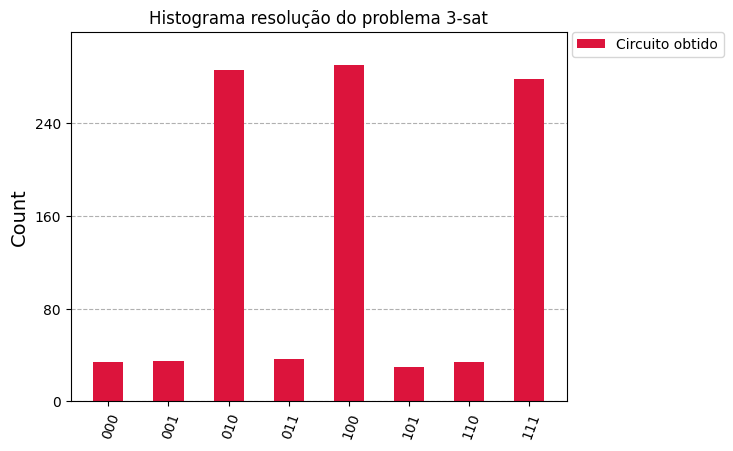
\includegraphics[width=\textwidth]{histograma_circuito_obtido.png}
        \caption{Resultados obtidos}
        \label{fig:histograma_circuito}        
    \end{subfigure}
    \begin{subfigure}{0.419\textwidth}
        \centering
        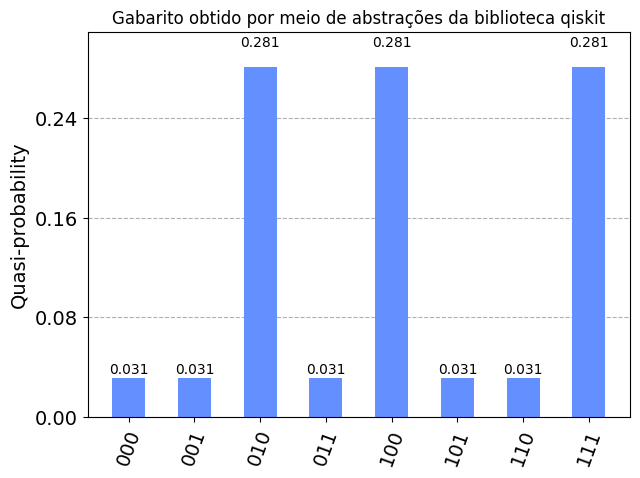
\includegraphics[width=\textwidth]{gabarito_qiskit.png}
        \caption{Gabarito}
        \label{fig:gabarito_qiskit}        
    \end{subfigure}
    \caption{Resultados de não satisfação da expressão FNC \ref{eq:expressao_fcn}}
\end{figure}

A fim de visualizar comparações com o estado da arte para a resolução do problema, foi utilizado uma implementação de abstrações de circuitos pré programados da biblioteca Qiskit como gabarito, resultando no histograma representado na figura \ref{fig:gabarito_qiskit}. Os resultados expressados nas figuras  \ref{fig:histograma_circuito} e \ref{fig:gabarito_qiskit} se encaixam perfeitamente nos valores de atribuição para C, B, A a fim de obter a satisfabilidade da equação, como comprovado na tabela verdade exposta em \ref{tab:tabela_verdade}
\begin{table}[h!]
\centering
\[
\begin{array}{|c|c|c|c|}
\hline
C & B & A & (\neg A \lor \neg B \lor \neg C) \land (A \lor \neg B \lor C) \land (A \lor B \lor \neg C) \\
\hline
\text{F} & \text{F} & \text{F} & \text{T} \\
\hline
\text{T} & \text{F} & \text{F} & \text{F} \\
\hline
\text{F} & \text{T} & \text{F} & \text{F} \\
\hline
\text{T} & \text{T} & \text{F} & \text{T} \\
\hline
\text{F} & \text{F} & \text{T} & \text{T} \\
\hline
\text{T} & \text{F} & \text{T} & \text{T} \\
\hline
\text{F} & \text{T} & \text{T} & \text{T} \\
\hline
\text{T} & \text{T} & \text{T} & \text{F} \\
\hline
\end{array}
\]
\caption{Tabela verdade da expressão FNC exposta na equação \ref{eq:expressao_fcn}}
\label{tab:tabela_verdade}
\end{table}

\section{Conclusões e trabalhos futuros}\label{sec:conclusoes}


Em conclusão, os resultados obtidos durante a aplicação deste artigo demonstram o potencial da computação quântica para a resolução de problemas clássicos, como no caso do 3-FNC-SAT. Em conjunto com as comparações realizadas na seção \ref{sec:resultados}, é possível afirmar que os resultados obtidos expressam uma solução ótima, cumprindo portanto o objetivo deste artigo de se resolver o problema proposto. 
A característica não determinística da computação quântica nos permite obter resultados de várias maneiras. Especificamente, o algoritmo de Grover provou ser uma ferramenta versátil para lidar não apenas com buscar em uma base dados, mas também para a solução de problemas NP completos como demonstrado no presente trabalho.

Em relação a trabalhos futuros, cabe citar alguns pontos que não foram destrinchados durante este trabalho, como por exemplo o cálculo da complexidade de tempo e espaço do circuito obtido e compará-lo com a computação clássica, ou então a possibilidade de se generalizar a quantidade de literais, a fim de resolver o problema k-FNC-SAT.
Também vale citar a possibilidade da criação de um circuito de classe P que tem como entrada um problema NP, e que ao ser executado o mesmo seria transitado para o problema do k-SAT a fim de por em prática sua NP completude comprovada por \cite{cook:71}. 

O código-fonte desenvolvido é de uso livre e está disponível em um repositório no \textit{Github}\footnote{
\url{https://github.com/gabrielms201/Quantum-Implementation-For-SAT-Problem-Solving}}.

\bibliographystyle{sbc}
\bibliography{sbc-template}
\end{document}